\documentclass{article}
\usepackage[utf8]{inputenc}
\usepackage{mathtools, amssymb, amsthm, amsmath} 
\usepackage{indentfirst}
\usepackage{chngcntr}
\usepackage{graphicx}
\graphicspath{./}
\usepackage{url}

% \title{Simulation of an Inverted Pendulum and Controller}
% \author{Eric Sherman}
% \date{April 29 2022}

\begin{document}

\begin{titlepage}
    \begin{center}
        \vspace*{1cm}
            
        \LARGE
        \textbf{Final Project - Simulation of a Inverted Pendulum and Controller}
            
        \vspace{0.5cm}
        \Large
        Computational Modeling and Simulation (ECE 1180)
        
            
        \vspace{0.5cm}
        \large
        Eric Sherman \\
        April 29 2022
        
        \vspace{2cm}
        % 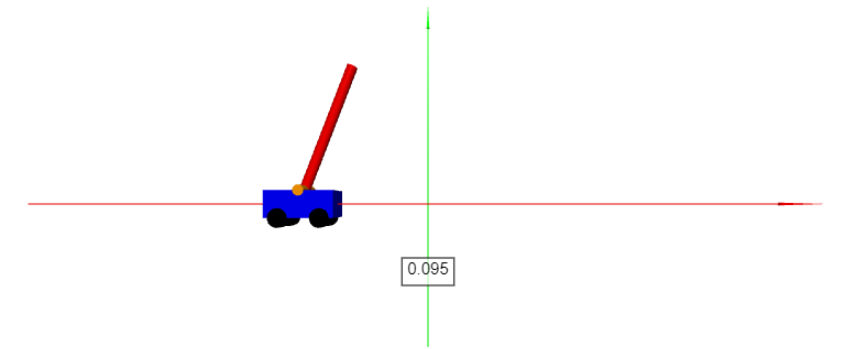
\includegraphics[width = 12 cm]{titlepage.png}
        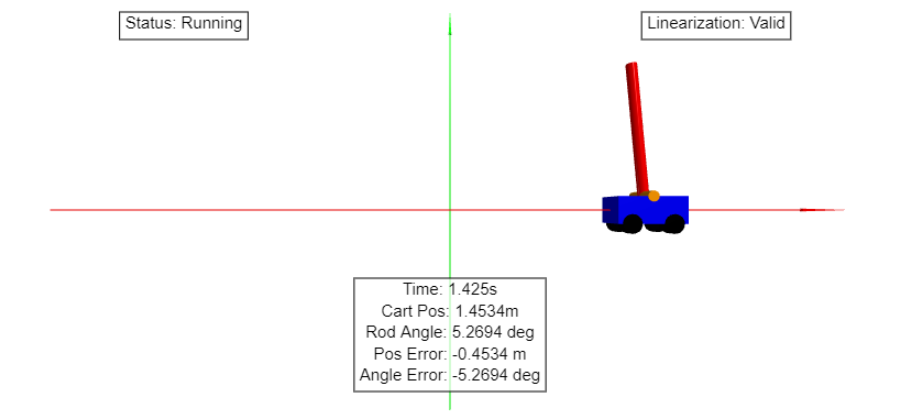
\includegraphics[width = 13 cm]{titlepage2.png}
            
        \vfill
        
    \end{center}
\end{titlepage}


\tableofcontents
\vfill


\section{Introduction}

In this project, I explore the dynamics of an inverted pendulums and potential methods to control it. An inverted pendulum is a rod-cart system. A cart (represented as a rectangular prism with 4 wheels attached) is restricted to just moving along the x-axis via push/pull force. A rod is a fixed to the top of the cart and is free to swing on a hinge that restricts the motion to just be along the x-y plane. The rod is allowed to swing the full 360 degrees meaning it is able to travel and clip through the cart.

The goal for the system is to achieve some final state (defined by the user) which usually calls for balancing the rod in the vertical upright position. This means that a controller had to be implemented because the system by itself is unstable. The rod will always fall over unless there is an external force applied to balance to the cart to position it in a way that prevents the rod from doing so. I've wanted to simulate this system for awhile now as it is a classic controls problem and I've seen it many times on social media, literature, and in lecture examples. Due to it's non-liner nature and being a single-input and multi-output system, there's many advanced control techniques required in order to be able to balance the rod in a perfectly vertical position. Several control methods were explored throughout this project including PID and state space control. 

\section{Motivation}

An inverted pendulum is a classic non-linear controls problem used in academia to teach state space representation, reinforcement learning, state space control, and linearization. My motivation behind this project was to scratch the surface of some of these controls and math topics by going through the full simulation of the system and the controller. Because everything about the system is simulated, an additional effort was needed to discretize the system and figure out the order in which to update the system state.

This model can be used to explore what happens when certain parameters of the system or the controller are changed and the performance of different controllers could be compared. Additionally, as an extension, the effect of disturbances or time delay can be visualized using this system as well. 

\section{Background}
\subsection{System Dynamics}

\begin{center}
    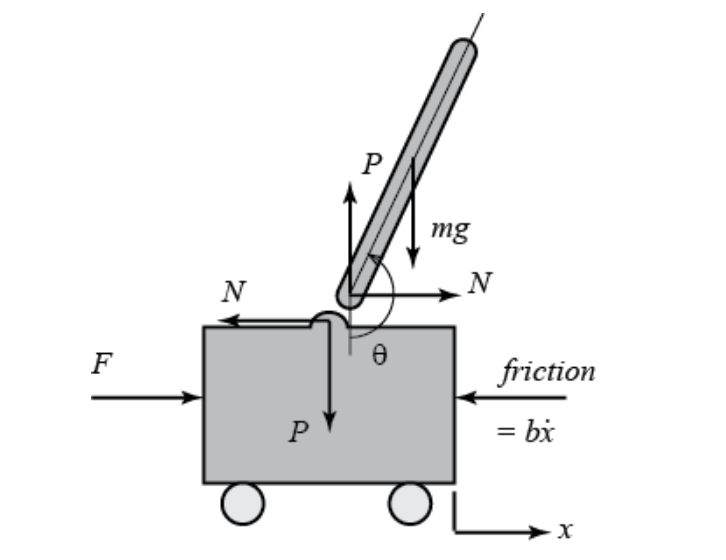
\includegraphics[width = 10cm]{Freebodydiagram.png} \\
    Figure 1. System model of the inverted pendulum. Source: [1]
\end{center}
\vspace{3 mm}

\noindent The cart-rod system is defined as follows:
\begin{enumerate}
    \item A cart is allowed to move latterly (restricted to x-axis) and is assigned a mass, $M$.
    \item The cart has friction in its wheels and this is simply modeled as \\ $F_{friction} = -b\Ddot{x}$ where $b$ is the coefficient of friction.
    \item A rod, attached to a hinge at the top center of the cart, is allowed to swing freely (full 360 degrees of motion in the x-y plane). There is no friction in the hinge.
    \item The rod has a mass $m$ and length of $2*l$, where $l$ is the distance to the center of the cart. It has a moment of inertia of $I$ given by $\cfrac{m(2l)^2}{3}$. It is important to remember that $l$ represents half the length of the rod as this is used throughout the calculations.
    \item The cart's x-position is represented by $x$. 
    \item The cart is pushed or pulled by a force $F$. 
\end{enumerate}

The equations can be derived using $F=m*a$ and $\tau = I* \alpha$. The dynamics are derived by summing all the forces in the horizontal direction for the cart, summing the horizontal forces on the rod, and then summing the forces on the perpendicular axis of the pendulum. This system is single-input and multi-output so there will be two dynamics equations needed to represent the whole system. The first equation comes from the horizontal forces on the cart and rod and the second equation comes from the forces on the on the pendulum. The focus of this project was more so on discretization of this system and on the controller, therefore I chose to use the equations provided by the University of Michigan in [1]. The derivation is also detailed in [2] and [3]. From [1], the final results are: 

\begin{equation}
    F = (M + m)\Ddot{x} + b\Dot{x} + ml\Ddot{\theta}\cos{\theta} - ml\Dot{\theta}^2\sin{\theta}
\end{equation}
\begin{equation}
    (I + ml^2)\Ddot{\theta} + mgl\sin{\theta} = -ml\Ddot{x}\cos{\theta}
\end{equation}

These equations are non-linear equations. Because most control methods can be applied to linear systems, it is required that these equations be linearized. Using the small angle theorem and other approximations and linearizing about the vertical equilibrium angle ($\theta = \pi$), we can greatly simplify the equations. These approximations are detailed in verification section. However, this means that in order for the system to be accurate, it must only operate within small angle deviations from $\theta = \pi$. Due to the linearization about  $\theta = \pi$, we define $\theta = \phi + \pi$ where $\phi$ is a small deviation from equilibrium.  After linearization (as detailed in [1]), the final equations become: 

\begin{equation}
    (I+ml^2)\Ddot{\phi} -  mgl\phi = ml\Ddot{x}
\end{equation}
\begin{equation}
    (M+m)\Ddot{x} + b\Dot{x} - ml\Ddot{\phi} = u
\end{equation}

Note that $F$ has been substituted with $u$ in equation (4) and will represent the input to the system or the force on the cart.

Since this system will be simulated, it is helpful to represent the system in an influence diagram. The elements in the system influence each other in the following ways:

\begin{center}
    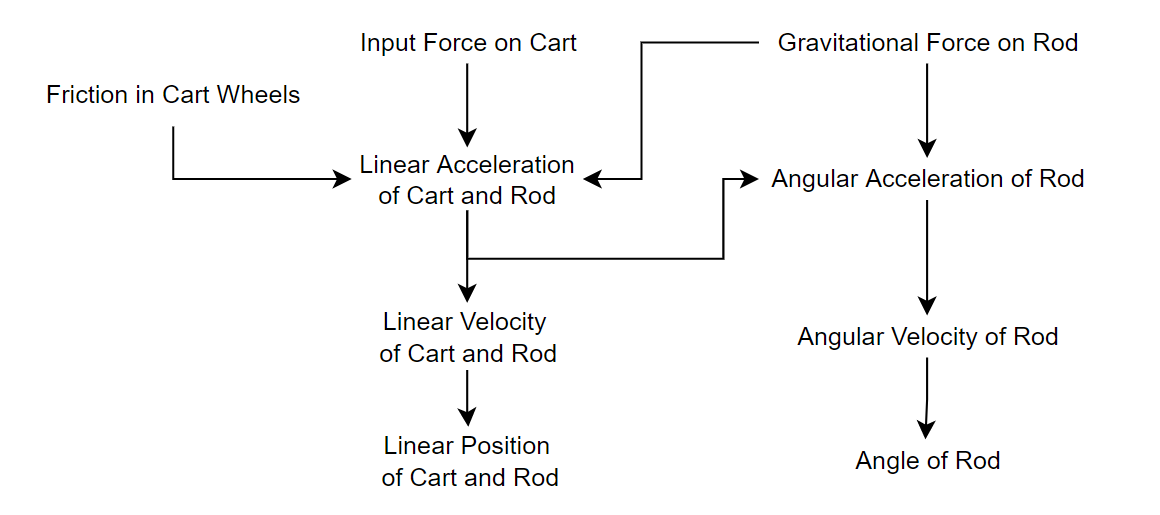
\includegraphics[width = 12cm]{influence_diag.png}
    Figure 2. Influence diagram for the inverted pendulum.
\end{center}

Continuing the derivation of the dynamics of the system, we can take the Laplace transform of these equations (as shown in [1]), yielding:

\begin{center}
    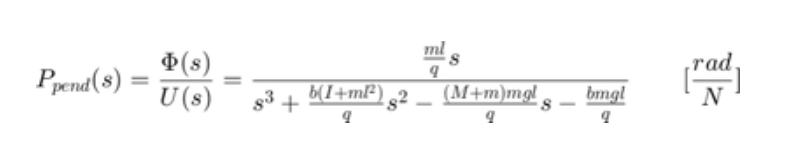
\includegraphics[width = 12cm]{transfer1.png}
    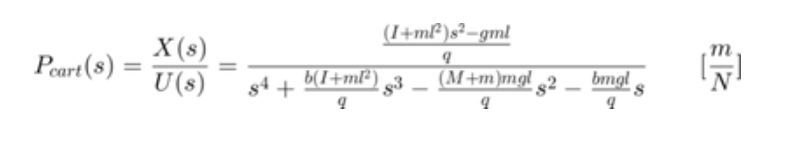
\includegraphics[width = 12cm]{transfer2.png}
    
\end{center}

where $q = (M + m)(I + ml^2) -(ml)^2$. If we take the inverse Laplace transform, we could see the functional relationships between the input and output for the system. As mentioned before, we have one input, the force, and two outputs, the position of the cart and the angle of the rod. The inverse Laplace transform of these functions would give us the time domain representation of the system and allow us to construct a simulation diagram representing the functional relationship between the input and the output. Because these systems are of higher order, completing this calculation would be complex. 


Since working with the time domain representation isn't feasible, I used state-space representation, which nicely models the system as a set of input and output matrices in the form of first order differential equations. The continuous-time state space representation is in the following form:

\begin{align}
    \Dot{x} = Ax + Bu \\
    y = Cx + Du
\end{align}

\noindent where A is the state matrix, B is the input matrix, C is the output matrix, D is the feed-forward matrix (in my case, just a zero matrix), x is the state vector, $\Dot{x}$ is the derivative of the x matrix, y is the output matrix, and u is the input matrix. For the inverted pendulum, the matrices are: 

\begin{center}
    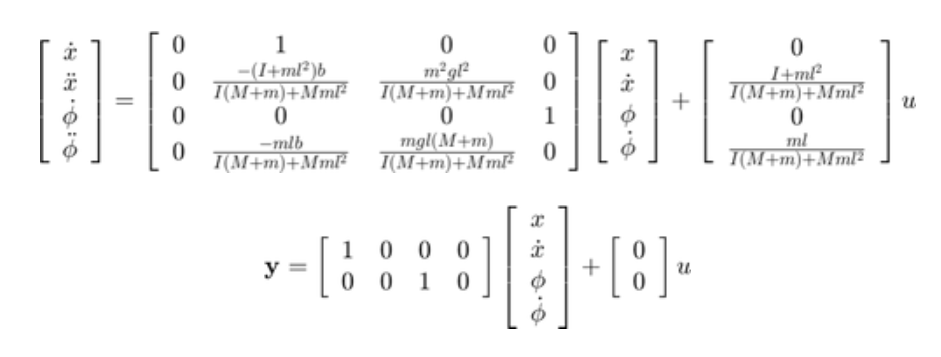
\includegraphics[width=12cm]{statespace.png}
\end{center}

The output $y$ is a 2x1 matrix where the first element is the cart's position and the second element is the deviation from the rod's equilibrium position. My simulation uses this state space representation in order to get next state values. 


\subsection{State Space Discretization}

In discrete time, the $\Dot{x}$ matrix is actually the next state matrix at $t + \Delta{t}$ instead of the derivative [8]. Using [7], we can discretize the state space representation:

\begin{align}
    \cfrac{dx}{dt} = \Dot{x} \approx \cfrac{x(k+1)- X(k)}{\Delta{T}}
\end{align}

\noindent where $\Delta{T}$ is the sampling interval. This approximation can be made only if $\Delta{T}$ is small. Simplifying: 

\begin{align}
    \cfrac{x(k+1)- x(k)}{\Delta{T}} & = Ax(k) + Bu(k) \\ 
    x(k+1) & = x(k) + A\Delta T x(k) + B\Delta T u(k) \\
    x(k+1) & = (I + A\Delta T)x(k) + B\Delta T u(k)
\end{align}

\noindent where I is the identity matrix:

\begin{equation}
    I = 
    \begin{bmatrix}
        1&0&0&0 \\
        0&1&0&0 \\
        0&0&1&0 \\
        0&0&0&1
    \end{bmatrix}
\end{equation}

\noindent and $x(k+1)$ contains the next state values. Equation (10) uses the forward Euler method. In my model, I use the backward Euler method changing Equation (10) to:

\begin{align}
    x(k+1) & = (I - A\Delta T)^{-1}x(k) + B\Delta T u(k)
\end{align}

\subsection{State Space Controller}

In this simulation, I used LQR (Linear Quadratic Regulator) as a controller. The use of a PID controller was explored but because this is a multi-output system, I would need to two PID controllers working in tandem. Therefore, LQR was a better option in this scenario.

LQR will produce a matrix of gains which is used in the update function:

\begin{equation}
    u = -Kx
\end{equation}

\noindent where x is the error, giving:

\begin{equation}
    u = -k(measured - setpoint)
\end{equation}

\noindent as detailed in Chapter 8 of [5]. K is in the from:

\begin{equation}
    K = 
    \begin{bmatrix}
        K_x & K_{\Dot{x}} & K_{\phi} & K_{\Dot{\phi}}
    \end{bmatrix}
\end{equation}

Both $measured$ and $setpoint$ are matrices with the same dimensions as the state matrix. In this case, $measured$ is just the state matrix, $x(k+1)$. We fill the setpoint matrix with the desired end states of the system. In my case, I want the final cart position to be 1 meter, the angle deviation of the rod to be 0, the cart velocity to be 0, and the angular velocity of the rod to be 0, although these can be modified in the code. This gives:

\begin{equation}
    setpoint = 
    \begin{bmatrix}
        1 \\
        0 \\
        0 \\
        0 \\
    \end{bmatrix}
\end{equation}

In order for LQR to produce the K matrix, we need the A and B matrix from earlier, and also a Q matrix and R value. R is the cost to control so if R is low, this means it doesn't cost much for us to actuate this system, meaning the controller will respond aggressively if needed. With a high R, this means the cost of controlling a system is high, so the controller will tend to be more conservative. The Q matrix contains weights for each of the state values. It is in the form:

\begin{equation}
    Q = 
    \begin{bmatrix}
        W_x & 0 & 0 & 0 \\
        0 & W_{\Dot{x}} & 0 & 0 \\
        0 & 0 & W_\phi & 0 \\
        0 & 0 & 0 & W_{\Dot{\phi}} 
    \end{bmatrix}
\end{equation}

\noindent where $W_x$, $W_{\Dot{x}}$,  $W_\phi$, and $W_{\Dot{\phi}}$ are weight values for each component of the system state. For example, if we want the controller to be really concerned about $W_\phi$, we would give it a value of 10 or 100. An optimal Q matrix I have found is:

\begin{equation}
    Q = 
    \begin{bmatrix}
        10 & 0 & 0 & 0 \\
        0 & 1 & 0 & 0 \\
        0 & 0 & 1000 & 0 \\
        0 & 0 & 0 & 10 
    \end{bmatrix}
\end{equation}

\noindent It is possible to make the controller unstable depending on your Q matrix. I have found that high position and velocity values for either the cart or the rod can result in unstable behavior because these states are directly related to each other.

Lastly, we add limits to the controller output ($u$) to prevent it from producing unreasonable forces on the cart. This limit can be modified in the $sim\_inputs$ class. 

\subsection{Simulation Update}

The update order is as follows:

\begin{enumerate}
    \item Get next state using $x(k+1)= (I + A\Delta T)x(k) + B\Delta T u(k)$
    \item Calculate the controller output using $u(k+1)= -K[x(k+1) - setpoint]$
    \item Calculate the new system output with the new u value, \\ $y(k+1) = Cx(k+1)+Du(k+1) $
    \item Update the simulation visuals and labels.
    \item Set $x(k)$ equal to $x(k+1)$, making the next value now the current state for the next loop iteration.
    \item Return to 1.
\end{enumerate}

\subsection{Selection of Model Parameters}

Most of the model parameters were used from [1]. I chose to lengthen the rod to make it easier to stabilize. Additionally, I chose a very small $\Delta t$ so that the discretization approximation is correct. At a high $\Delta t$ values, the system will become unstable. 

In terms of the controller, I tuned the Q matrix until I was able to get an optimal response. The R value I chose to be fairly low because in a simulation, it doesn't cost anything to actuate the system.

Additionally, I chose to add an initial rod offset and an initial force so that the controller has to immediately kick into action to prevent the rod from turning over. I added two customizable disturbances in the form of a cart disturbance and a rod disturbance later on the simulation. It is important that I chose initial values that prevents the rod from having a large enough deviation that the angle approximations are no longer accurate. If this happens, the system behavior might be incorrect. I implemented a check to warn the user if the rod falls out of the region of nominal operation.


\section{Verification}

\subsection{Controllability}
We first check the controllability of the system using the methods detailed in [4]. I implemented a function to complete this check at the start of the simulation and print the result. The ctrb() function takes the A and B matrix as an input. For the A and B matrices used in this project, the system is controllable.

\subsection{Linearization Checks}
Because this is a linearized non-linear system, checks were implemented to ensure that the system operated within a region where the linearization was still accurate. In the top right corner of the simulation, a label displays whether the linearization is still accurate or not.

The following linearizations were used (from [1]):

\begin{align}
    \cos{\theta} = \cos{(\pi + \phi)} &\approx -1 \\
    \sin{\theta} = \sin{(\pi + \phi)} &\approx -\phi \\
    \Dot{\theta}^2 = \Dot{\phi}^2 &\approx 0 \\
\end{align}

\noindent These linearizations are shown below:
\vspace{5mm}

\begin{center}
    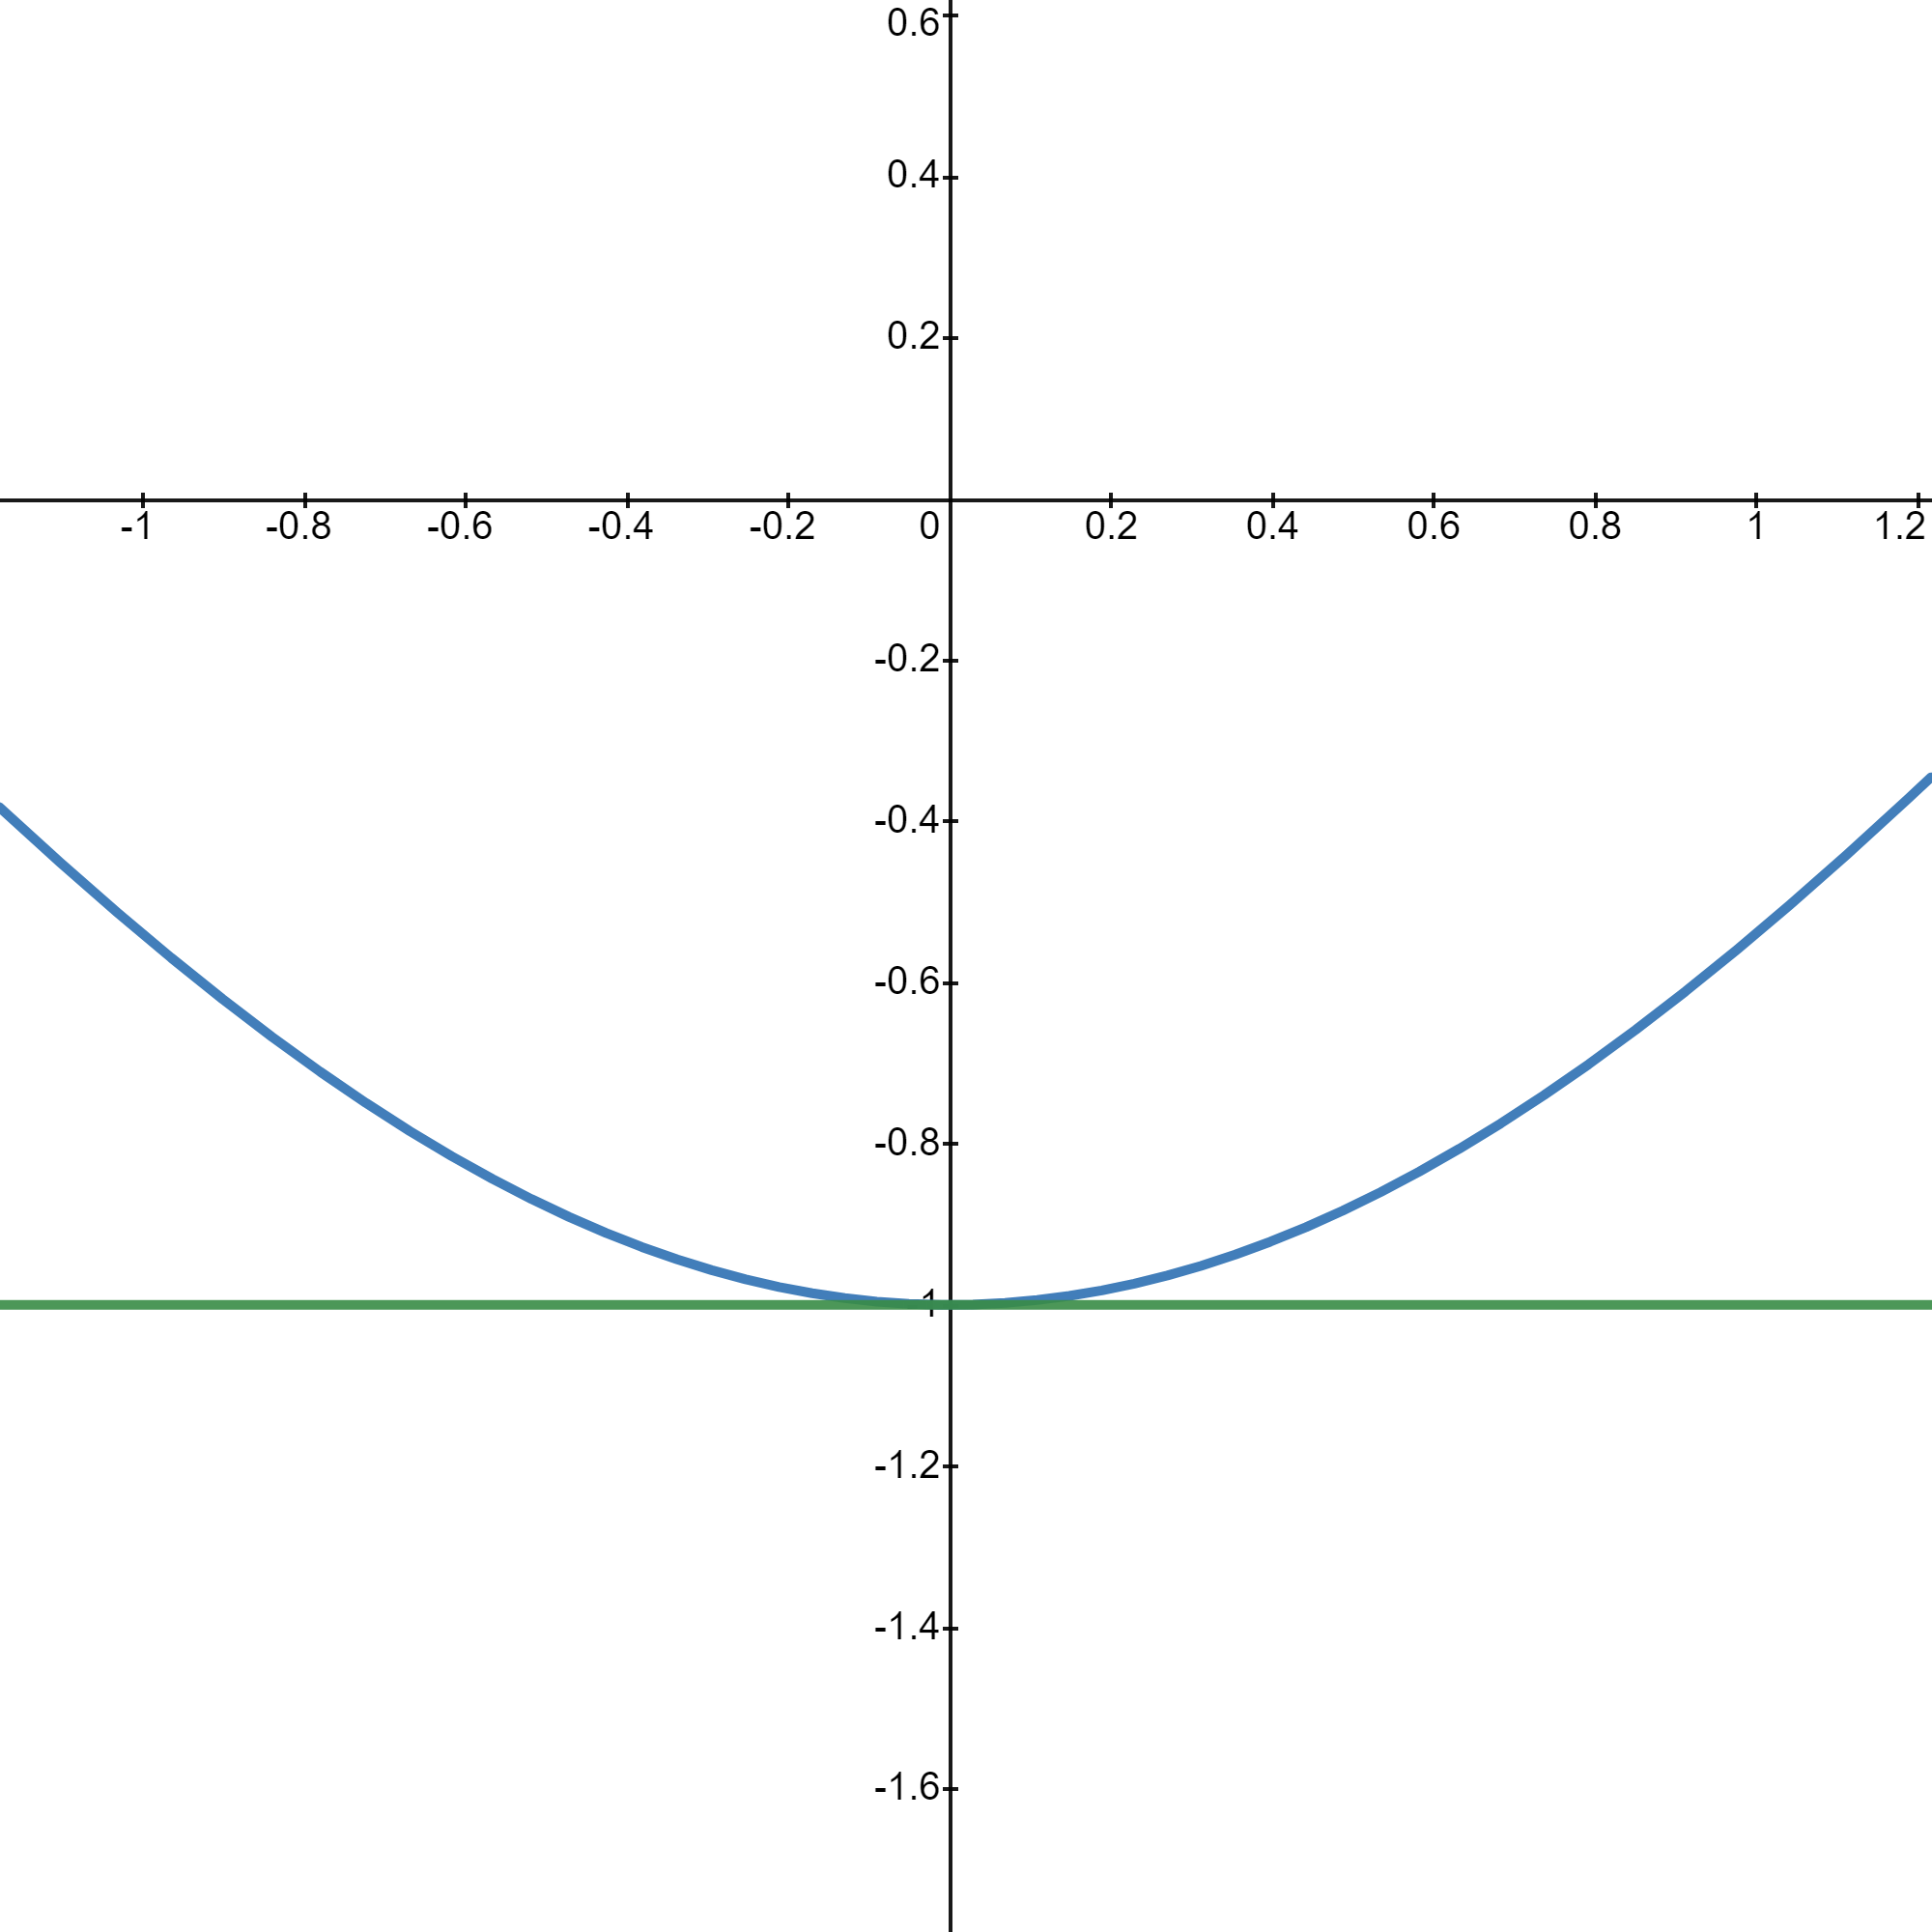
\includegraphics[width = 8cm]{cos-linear.png}\\
    Figure 3. Cosine approximation. \\
    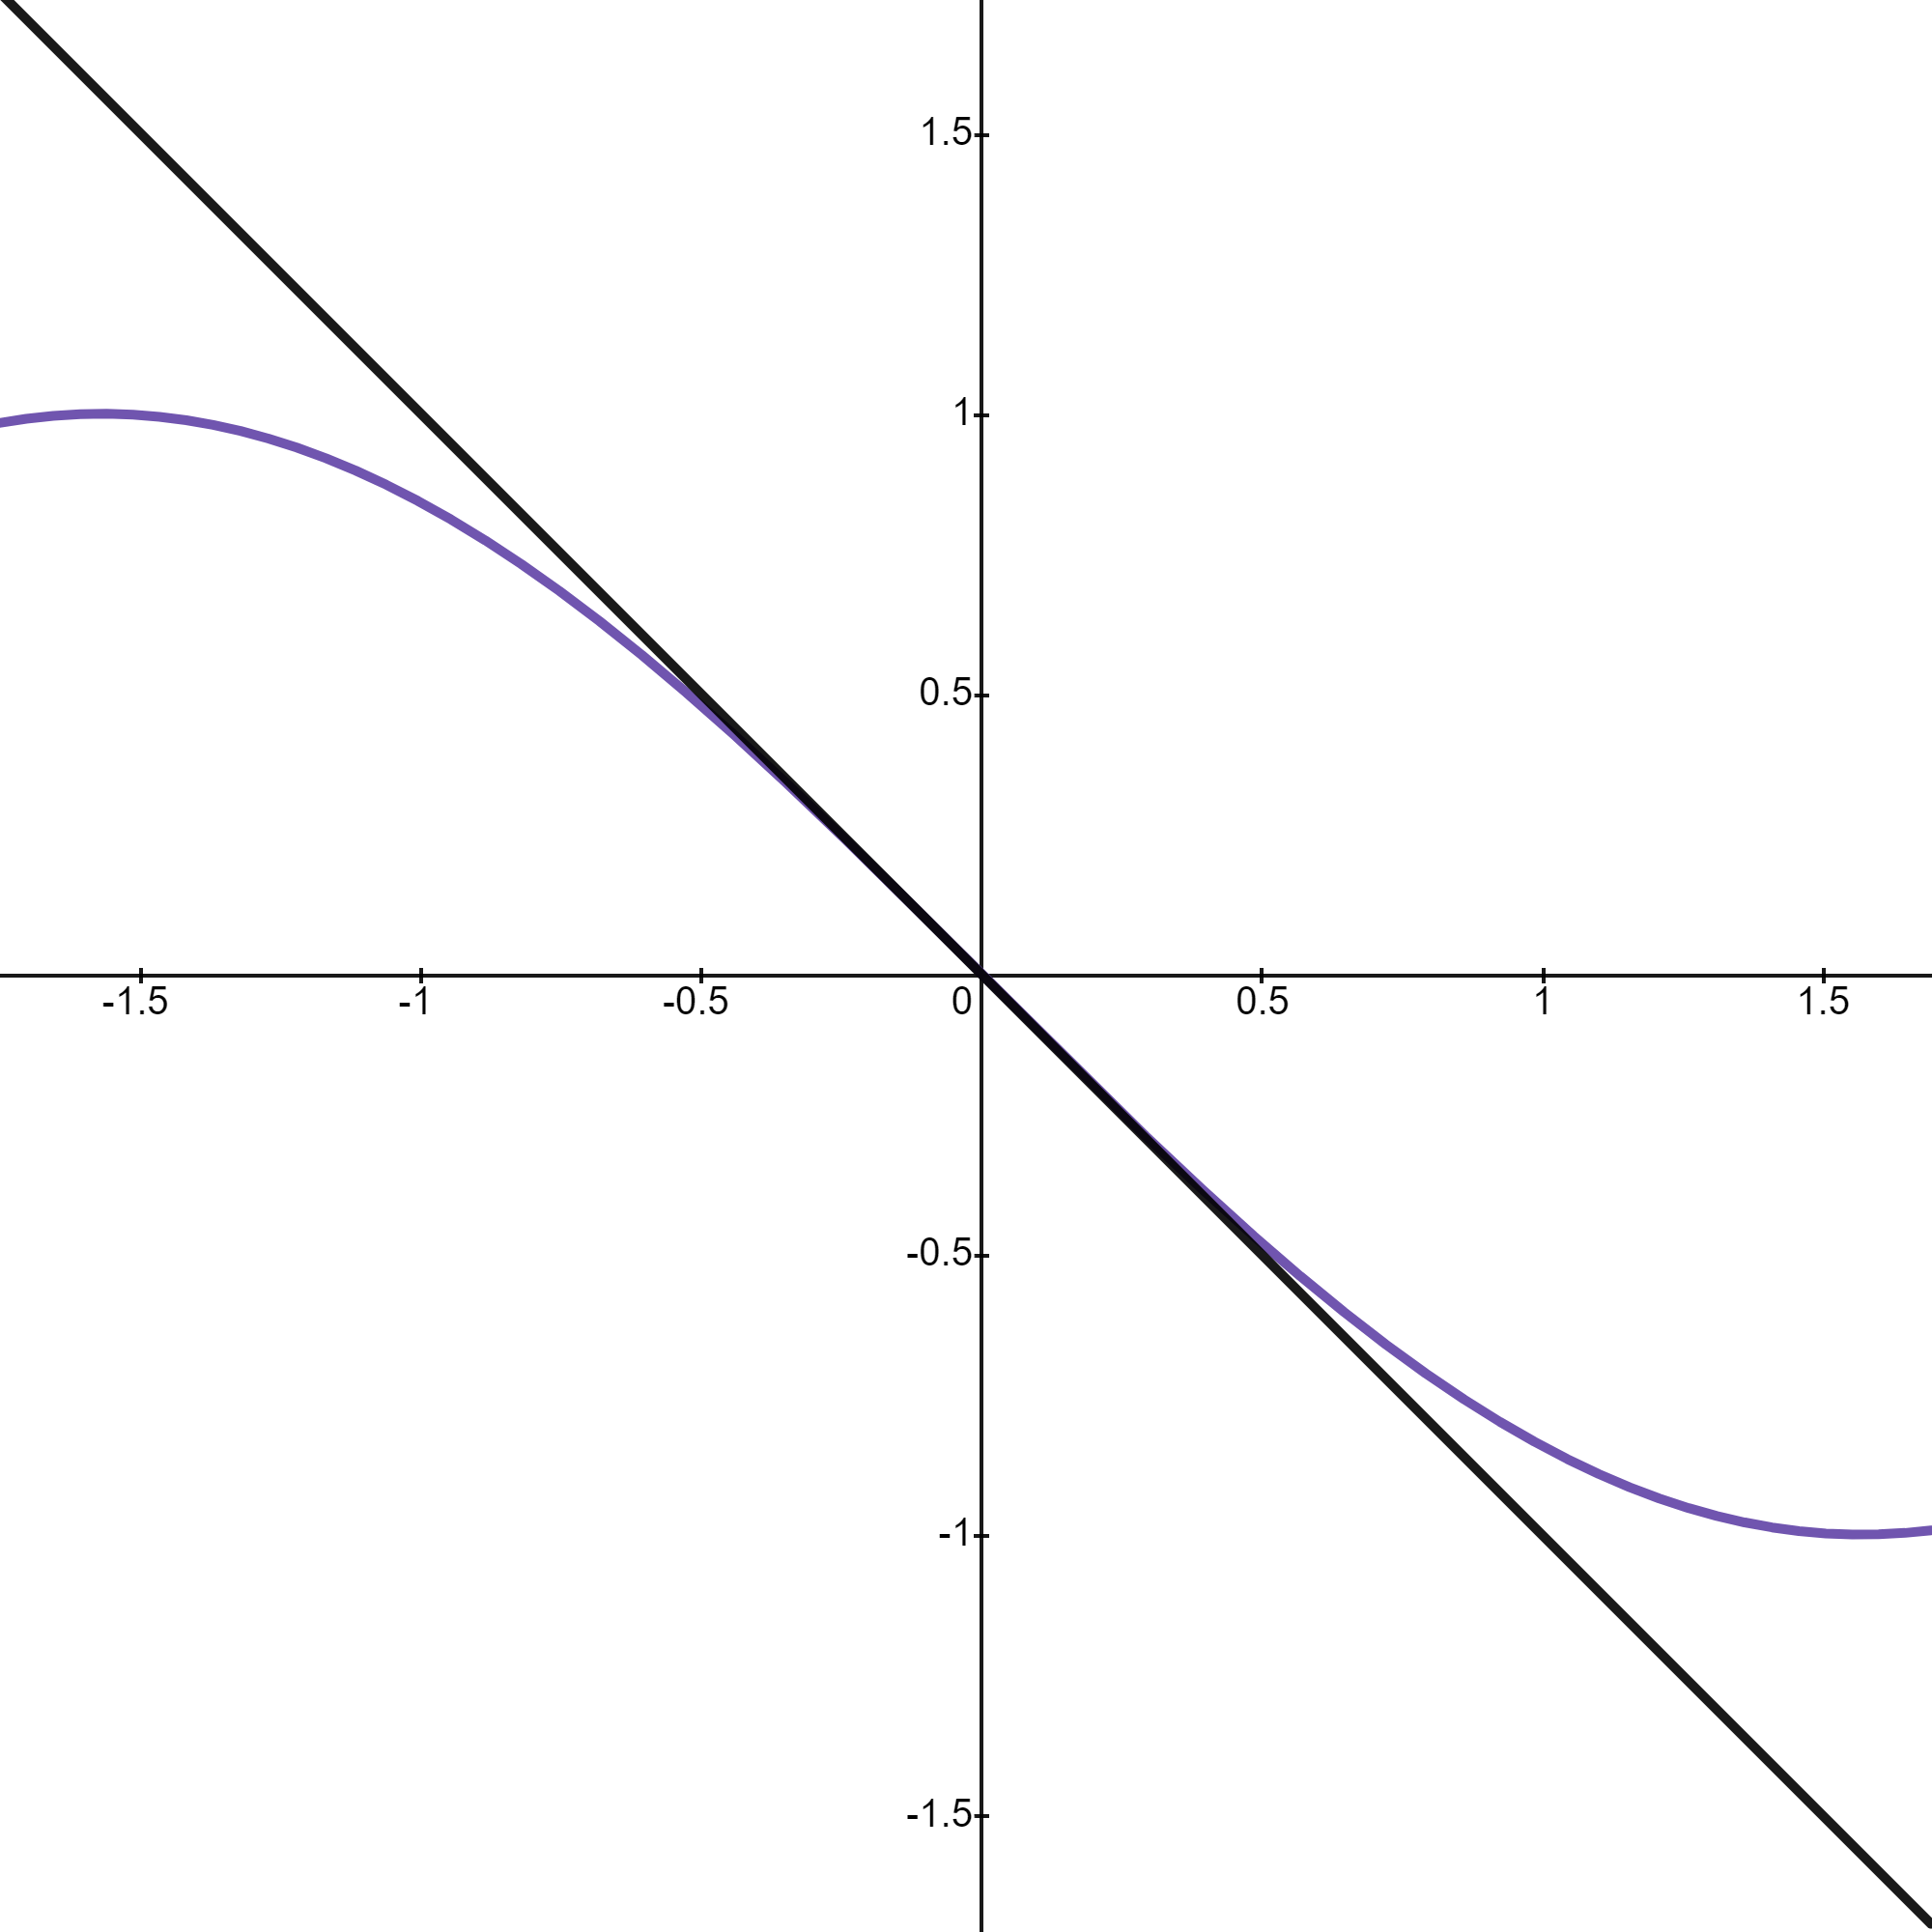
\includegraphics[width = 8cm]{sin-linear.png} \\
    Figure 4. Sine approximation. \\
        \vspace{8mm}
    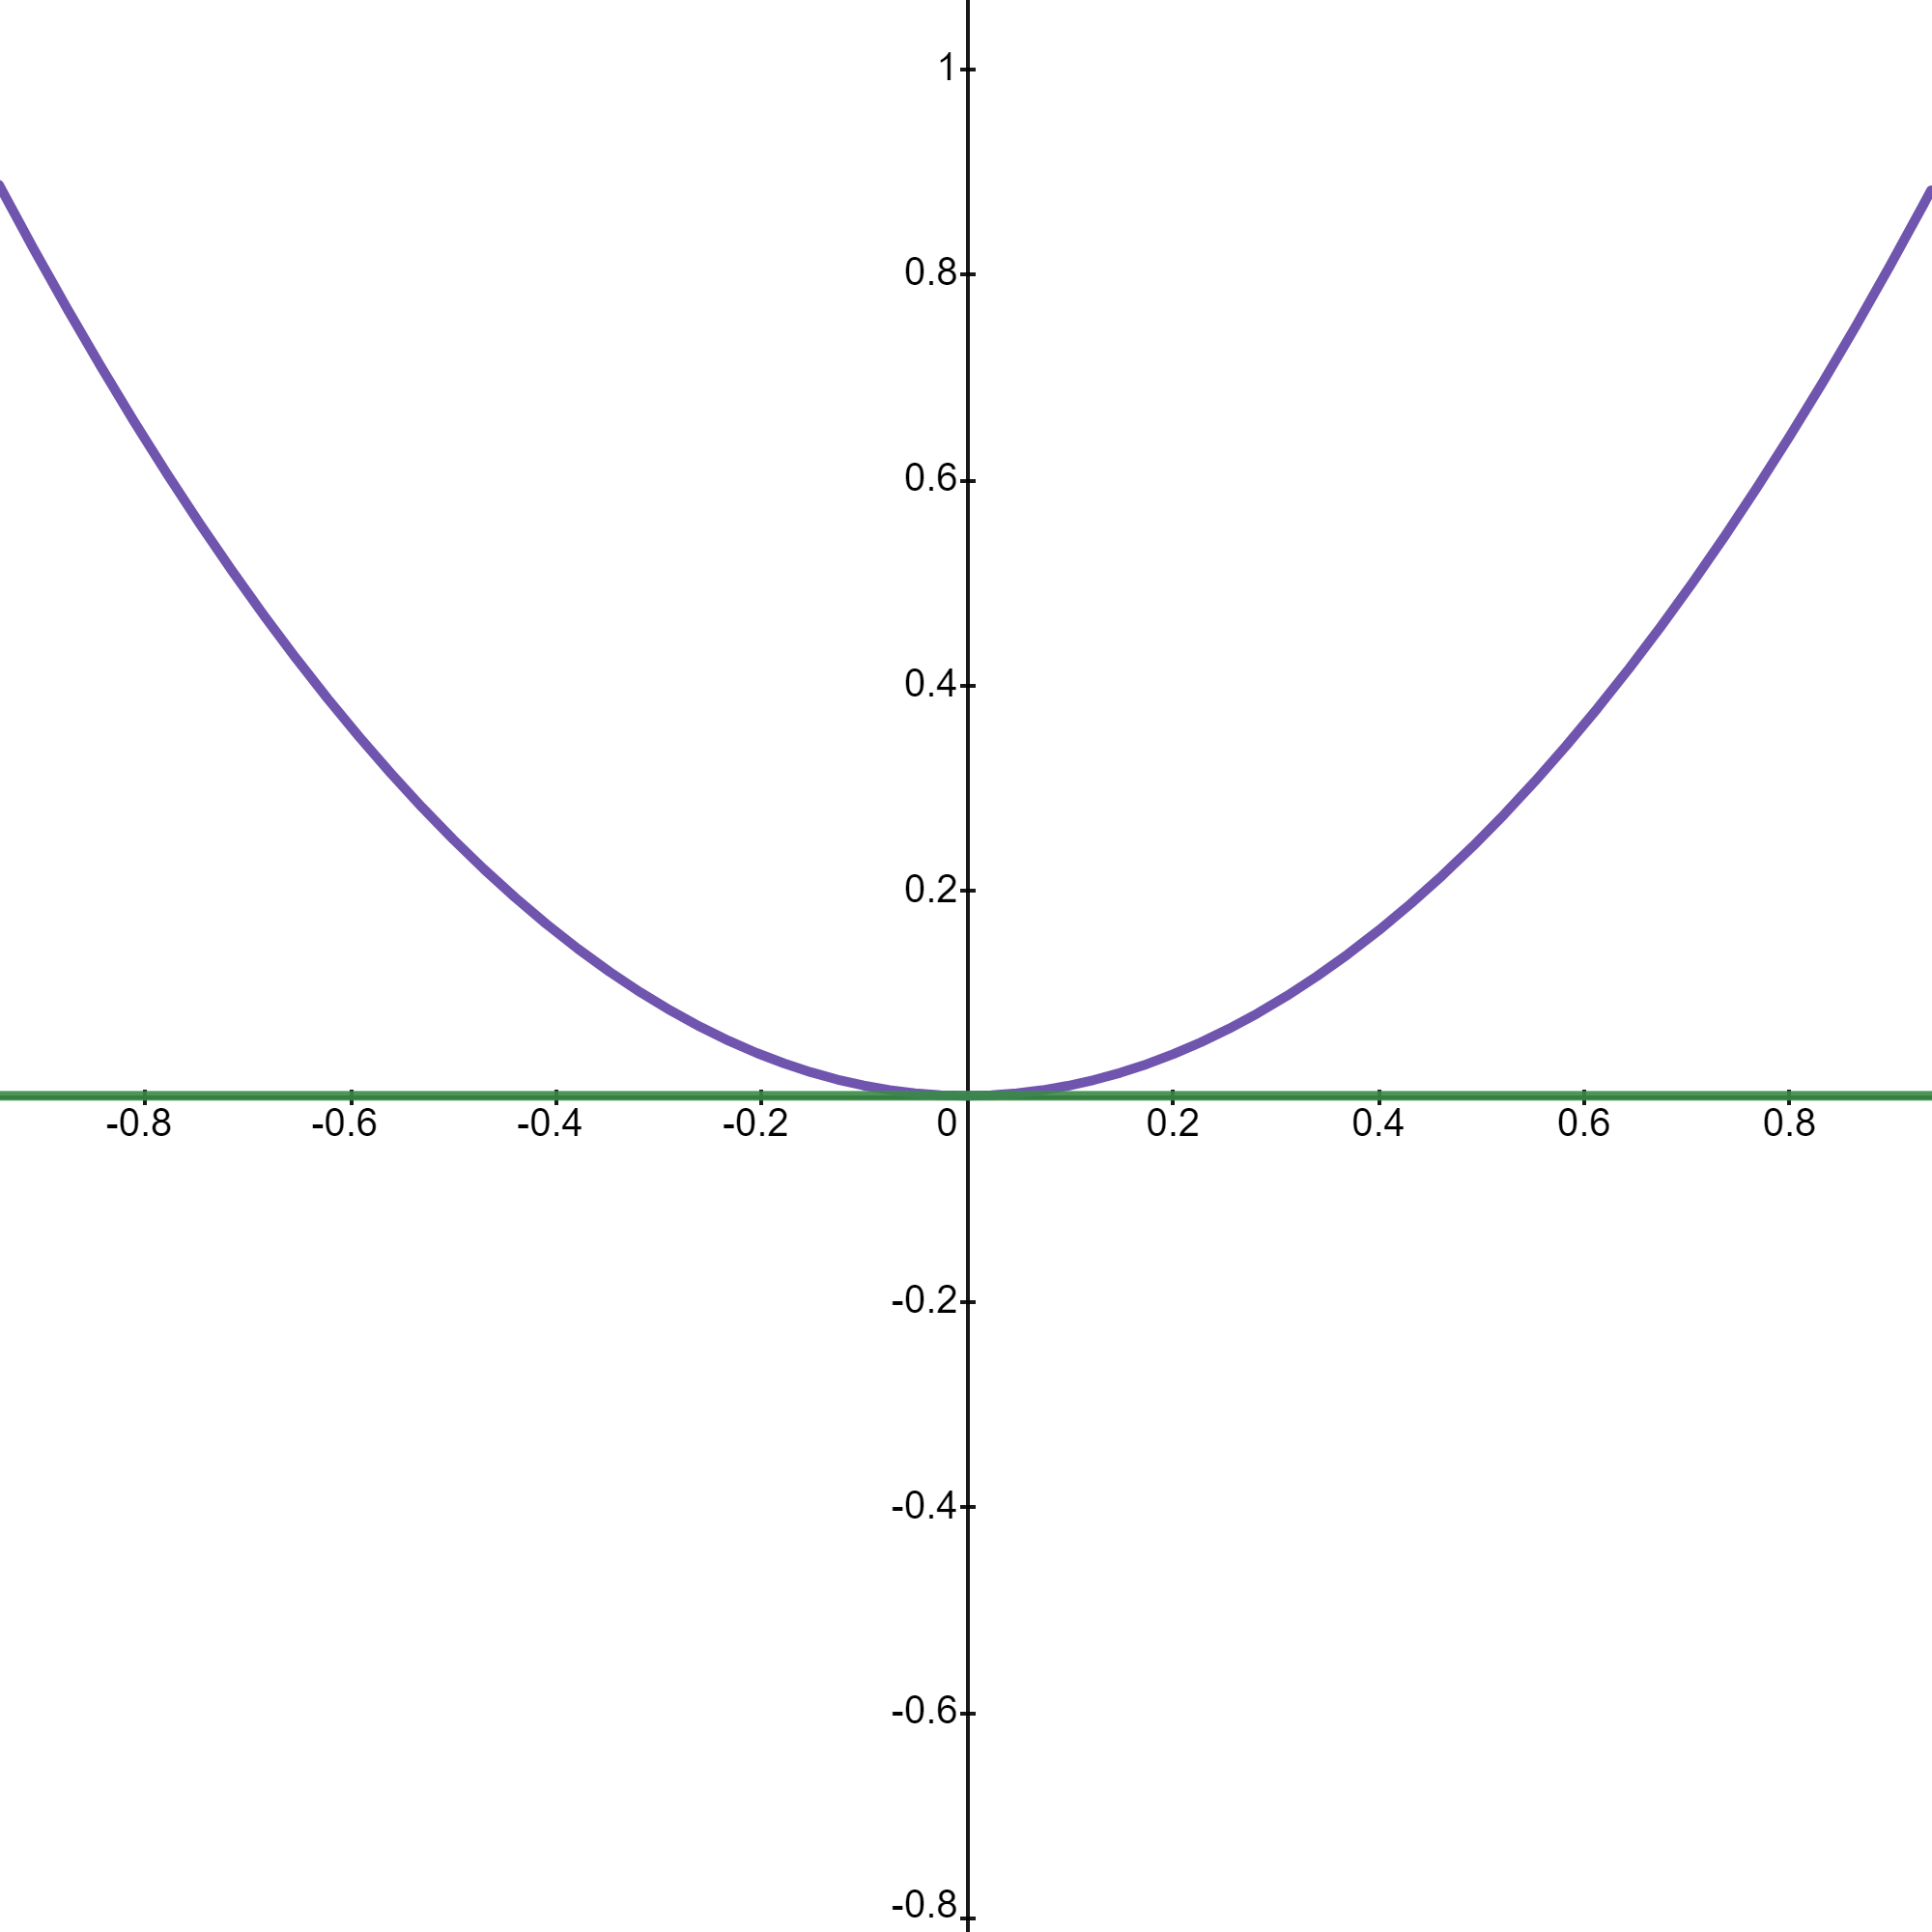
\includegraphics[width = 8cm]{squared-linear.png} \\
    Figure 5. $\Dot{\phi}^2$ approximation. \\
\end{center}

I set 20\% error as the threshold for considering the approximations accurate. The fastest approximation to hit this threshold is  $\Dot{\phi}^2$. This occurs when the absolute value of the angle is 0.45 radians.

\subsection{Visual Verification}

The simulation behaves as expected and can balance the rod upright, even after several different disturbance profiles such as an impulse disturbance in the rod angle, an impulse disturbance in the cart force, and a rectangular pulse disturbance in the cart force (applying the same force over time for x seconds). As long as the initial disturbances aren't too great and the angle deviation for the rod stays close to the equilibrium point, the system model is accurate and the controller behaves as expected.

A comparison of this model and other models can be used as well. It is important to note that most other models use a mass-less rod with a point mass at the end. This changes the dynamics significantly. Under the "Python (GEKKO) Solution" in [11], we can see the response for the pendulum system with an initial force on the cart to the left. I have attempted to reproduce this using the parameters under "Verification" in the Scenarios section. The initial response of both systems is almost identical. However, with my system, the cart adjusts for the rod angle error immediately. Unfortunately, if I have reduce the weight for the rod angle error, I will get bad oscillations as the cart tries to reach the set position. If I increase the weight for the rod angle error, then the cart will follow a different trajectory than in [11]. Because the models used aren't exactly identical, this discrepancy in the trajectory of the rod and cart towards the end of the motion is expected. However, both models properly reach the desired end state.

Other sources that have been used to verify my simulation and ensure that my model and implementation are correct has been outlined throughout the Background section.

\section{Scenarios}

Here, I have listed sets of initial values that result in different controller responses. These parameters can be found in $plant\_inputs$ or the $sim\_inputs$ class. An * next to the name means that this scenario has been used for verification. If a parameter is not listed, this means the original simulation values were used. This includes things such as cart mass, rod length, rod mass, etc. In scenarios in which disturbances are a part of, I have included the disturbance parameters. If the they are omitted, the following parameters are assumed to be set: rod\_disturbance\_on = False and cart\_disturbance\_on = False. However, these parameters and related disturbance parameters are not hard requirements can be modified by the user if desired.

\begin{enumerate}
    \item Stable Oscillatory Response
        \begin{itemize}
            \item end\_state = np.array([[0], [0], [0], [0]])
            \item weights = [100, 1, 1000, 1]
            \item cart\_starting\_pos\_x = -1
            \item rod\_starting\_angle = 0
            \item init\_force = -500
            \item max\_force\_limit = 10
            \item min\_force\_limit = -max\_force\_limit
        \end{itemize}
        
    \item Unstable Oscillatory Response
        \begin{itemize}
            \item end\_state = np.array([[0], [0], [0], [0]])
            \item weights = [100, 1, 1000, 1]
            \item cart\_starting\_pos\_x = -1
            \item rod\_starting\_angle = -math.pi/7
            \item init\_force = -500
            \item max\_force\_limit = 10
            \item min\_force\_limit = -max\_force\_limit
        \end{itemize}
        
    \item Triple Disturbance 
         \begin{itemize}
            \item end\_state = np.array([[1], [0], [0], [0]])
            \item weights = [10, 1, 1000, 10]
            \item cart\_starting\_pos\_x = -1
            \item rod\_starting\_angle = -math.pi/7
            \item init\_force = 800
            \item max\_force\_limit = 10
            \item min\_force\_limit = -max\_force\_limit
            \item rod\_disturbance\_on = True
            \item rod\_disturbance\_at\_time = 7
            \item rod\_disturbance\_angle = -math.pi/6
            \item cart\_disturbance\_on = True
            \item cart\_disturbance\_at\_time = 10
            \item cart\_disturbance\_force = 9
            \item cart\_disturbance\_over\_num\_steps = 30
        \end{itemize}
    
    \item Unstable Controller (saved by limits)
        \begin{itemize}
            \item end\_state = np.array([[1], [0], [0], [0]])
            \item weights = [1, 1, 1000, 100]
            \item cart\_starting\_pos\_x = -1
            \item rod\_starting\_angle = -math.pi/7
            \item init\_force = 0
            \item max\_force\_limit = 10
            \item min\_force\_limit = -max\_force\_limit
        \end{itemize}
        
    \item Verification *
        \begin{itemize}
            \item end\_state = np.array([[0], [0], [0], [0]])
            \item weights = [30, 1, 200, 10]
            \item cart\_starting\_pos\_x = -1
            \item rod\_starting\_angle = -math.pi/12
            \item init\_force = -300
            \item max\_force\_limit = 10
            \item min\_force\_limit = -max\_force\_limit
        \end{itemize}

\end{enumerate}

\section{Results}

Here, the results from different scenarios highlighted above will be included. The initial conditions for each scenario is specified above.

On the output graph, the control output (force in Newtons) is in red, the angle from vertical (degrees) is in blue, the cart position in meters is in purple, and lastly, linearization valid is an orange curve that is equal to 0 if the linearization is no longer valid or equal to the 25.7831 if the linearization is valid. 25.7831 (degrees) is the threshold between valid and invalid.

\subsection{Scenario: Stable Oscillatory Response}

    \begin{center}
        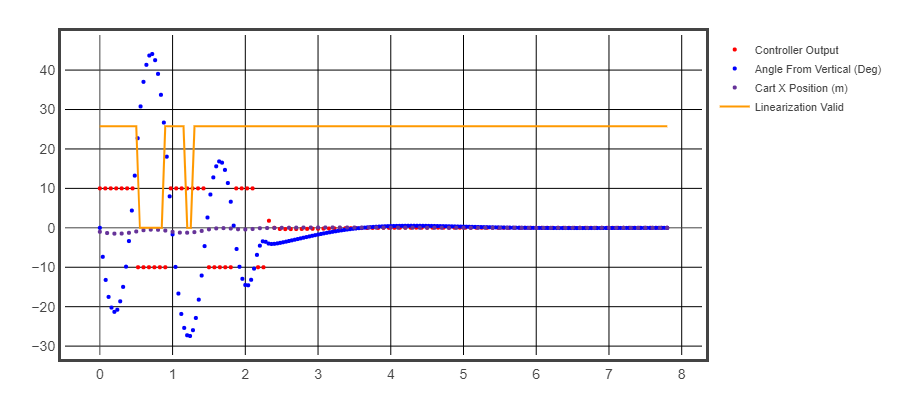
\includegraphics[width=15cm]{stableoscillationresponse.png}
        Figure 6. Unstable Oscillation. 
    \end{center}
    
    This response showcases what happens when the system is close to being unstable. We can see that the rod frequently swings out of the region where the linearization is valid.

\subsection{Scenario: Unstable Oscillatory Response}

    \begin{center}
        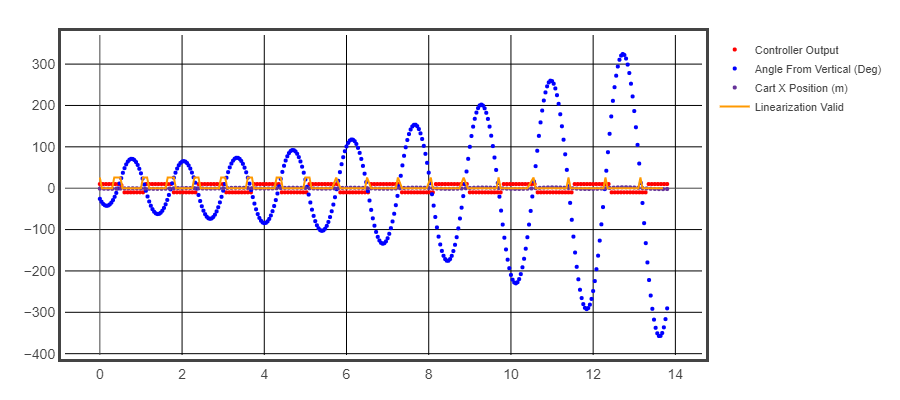
\includegraphics[width=15cm]{Unstableoscresponse.png}
        Figure 7. Unstable Oscillation. 
    \end{center}
    
    Here, the angle deviation grows exponentially. We can see that the linearization is invalid for all of the time besides when the rod swings back past the equilibrium. The controller output is saturated for the entire simulation as well.
    
\subsection{Scenario: Triple Disturbance}    
    \begin{center}
        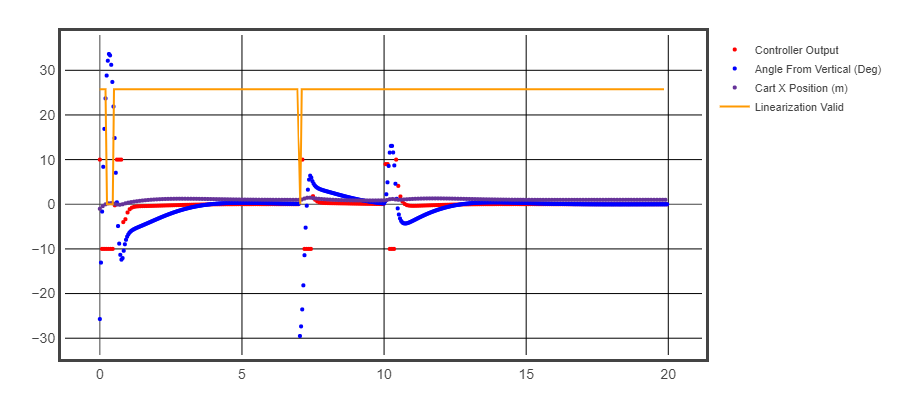
\includegraphics[width=15cm]{triple disturbance.png}
        Figure 8. Triple disturbance scenario.
    \end{center}
    
     The system settles quickly and rarely operates outside of the safe region (the region where linearization approximations still apply). The controller quickly counteracts the disturbances at t=7 and t=10.
    
    
\subsection{Scenario: Unstable Controller}
    \begin{center}
        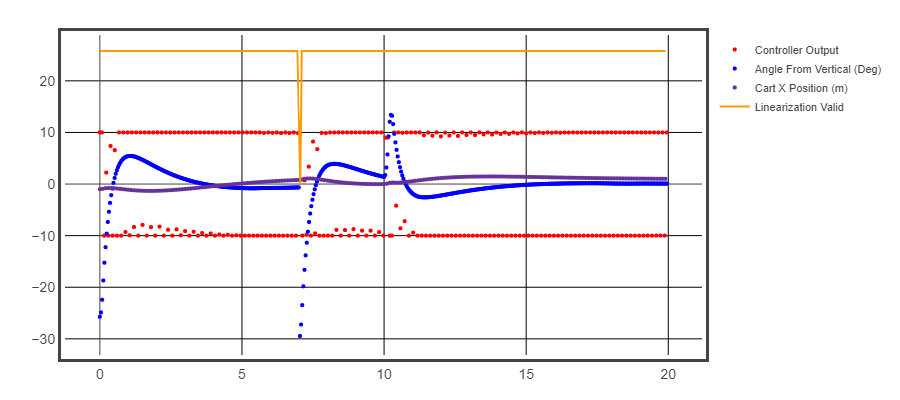
\includegraphics[width = 15cm]{unstablecontroller.png}
        Figure 9. Unstable controller scenario (disturbances included).
    \end{center}
    
    The controller mostly acts as a bang-bang controller due it continually jumping from its positive limit to its negative limit and vice versa. Without limits, the controller output explodes to $\infty$. This is because two output states of the system that are directly related were set to a high weight. Because of this direct relationship, the controller is unable to respond sensibly.
    

\section{Evaluation}

\subsection{Results}

The Results section highlights the potential effects to the system due to different system inputs. With unreasonable weights, or with initial input forces or rod angles that result in pushing the system out of the safe region, we begin to get odd behavior. This is reflected in the results. 

\subsection{Model Limitations}

As discussed above, several approximations are used in the simulation. To start, the system had to be linearized in order to make it compatible with most controllers. As such, if the rod moves to an angle where these linearization approximations are no longer accurate, then the system is no longer accurate and odd behavior may occur. This is discussed in more detail in section 4.2. 

Another limitation is the discretization approximation. As shown in section 3.2, equation (7), this approximation can only be made if $\Delta T$ is small. As tested but not included in this report, a $\Delta T$ of 0.01 instead of the chosen nominal time of 0.005 seconds results in an unstable system.

\subsection{Reflection}

This model is best setup to explore tuning of controllers and exploring behavior when the system is pushed beyond its limits. This model can be an excellent leaerning example covering many controls and math concepts such as linearization, state space representation, state space control, and discretization.

Throughout this project I encountered many challenges. My first big challenge was discretizing the state-space representation so that I could use the model provided by [1] in my simulation. The second big challenge was finding and tuning a controller that worked for this application. I began with a PID controller; however, this is a difficult solution to implement for this type of problem. This is because this system is single-input, multi-output whereas PID is only single-input, single output. A PID solution to this problem would probably require two PID controllers. I spent quite some time trying to implement this approach but after some digging and coming across state-space controllers, I decided to abandon that effort. The last big challenge was figuring out the correct order in which to update the system and the controller. Thank you Dr. Mao for assisting me with this. The remaining bulk of my time was figuring out minor bugs such as accidentally setting gravity to be 9.8 instead of -9.8, figuring out that certain assignments of weights can make the controller extremely unstable, and lastly, discovering that my model was using the wrong equilibrium point (credits to Dr. Mao again for this catch). Utilizing many Wikipedia articles, assistance from peers and Dr. Mao, I was able to take the project to a working state.

Some other approaches that I could have taken towards the modeling is using different differentiation approaches. For example, using the Runge-Kutta method, forward Euler, or the bilinear transform (Tustin's method) would have likely worked as well. Another approach is to directly operate on the non-linear dynamics using a differential nonstiff solver such as ode45 (implemented in MATLAB).

\section{Conclusions and Future work}
\subsection{Conclusion}

In this project, we explored the development of a model and representation of an inverted pendulum - cart system. The model had to be linearized in order to use a controller. We also explored the development this controller and tuning it to get the desired response. We went through several scenarios which highlighted different controller and system responses.

\subsection{Future Work}
In terms of future work, I would like to analyze the effects of introducing different delays in the controller feedback. At a large enough time delay, the system should become unstable. Additionally, I would like to explore using other controllers with this system or even taking a machine learning approach - for example, using reinforcement learning. 

As an extension, it would be interesting to potentially explore a system that is not bound to a 2D plane for both the cart and the rod.

\section{Acknowledgements}
\noindent A big thank you to:
\begin{itemize}
    \item Dr. Zhi-Hong Mao, for helping me discretize state space representation and assisting with debugging the controller.
    \item Thomas Detlefsen for helping me learn state space representation.
    \item Matthew Sivaprakasam for assisting with implementing and debugging a PID controller approach.
    \item Dr. Kara Bocan for providing advice and direction on the project.
\end{itemize}


\section{References}

\noindent $[1]$ Inverted Pendulum, System Modeling: \url{https://ctms.engin.umich.edu/CTMS/index.php?example=InvertedPendulum&section=SystemModeling}
\\
\vspace{1 mm} \\
$[2]$ Inverted pendulum: \url{https://en.wikipedia.org/wiki/Inverted_pendulum}
\\
\vspace{1 mm} \\
$[3]$ LCS - 13 - Pendulum on cart system - mathematical modeling and transfer function: \url{https://www.youtube.com/watch?v=c3z4eo6s0Ek}
\\
\vspace{1 mm} \\
$[4]$ Controllability and Observability: \url{https://www.ece.rutgers.edu/~gajic/psfiles/chap5traCO.pdf} \\
\\
$[5]$ Data Driven Science and Engineering; Machine Learning, Dynamical Systems, and Control: \url{http://databookuw.com/databook.pdf} \\
\\
$[6]$ Modeling and Simulation of Inverted Pendulum: \url{https://www.cantorsparadise.com/modelling-and-simulation-of-inverted-pendulum-5ac423fed8ac}
\\
\vspace{1 mm} \\
\noindent $[7]$ Discretization: \url{https://en.wikipedia.org/wiki/Discretization} \\
\vspace{1 mm} \\
$[8]$ State-Space Representation: \url{https://en.wikipedia.org/wiki/State-space_representation} \\
\vspace{1 mm} \\
$[9]$ Simulating and controlling an inverted pendulum: \url{https://fab.cba.mit.edu/classes/864.17/people/copplestone/final_project/index.html} \\
\vspace{1 mm} \\
$[10]$ Linear Quadratic Regulator (LQR) Control for the Inverted Pendulum on a Cart [Control Bootcamp]: \url{https://www.youtube.com/watch?v=1_UobILf3cc} \\
\vspace{1 mm} \\
\noindent $[11]$ Inverted Pendulum Optimal Control: \url{https://apmonitor.com/do/index.php/Main/InvertedPendulum} \\
\vspace{1 mm} \\
$[12]$ Full-state Feedback Control: \url{http://web.mit.edu/16.31/www/Fall06/1631_topic13.pdf} \\
\vspace{1 mm} \\
$[13]$ State-Space Models and the Discrete-Time Realization Algorithm: \url{http://mocha-java.uccs.edu/ECE5710/ECE5710-Notes05.pdf} \\

\end{document}
